\section{Introduzione}
La presente tesi mira a studiare come cambia la vegetazione nel fiume Tagliamento in risposta al regime idrologico (successione di magre, piene \emph{bankfull}, \emph{flood pulses}).
L'obiettivo principale è quello di ricercare una relazione che leghi i livelli del pelo libero dell'acqua registrati da un idrometro con la quantità di vegetazione erosa in seguito ad una piena, o che leghi i livelli con la quantità di legname che si ritrova in alveo dopo eventi di piena.
In via previsionale si cerca di rispondere all'esigenza di stimare in anticipo gli effetti sulle isole che può avere una piena in questo fiume.
\\
Inoltre si trovano traiettorie evolutive per quanto riguarda la larghezza e la percentuale di isole rispetto all'alveo attivo, anche confrontando i dati ottenuti per un tratto di qualche chilometro con alcuni risultati da letteratura; si ottengono relazioni tra la forza della corrente (\emph{stream power}) e la quantità massima di isole presenti.
%Inoltre si trovano valori soglia del livello del pelo libero per l'erosione della vegetazione.
%\\
%Dalla quantificazione dell'erosione della vegetazione dovuta alle piene, della quantità di legno in alveo e di un tasso di crescita della vegetazione si tenta di costruire un bilancio di materia vegetale a scala di evento di piena.

Si analizzano immagini satellitari e ortofoto al fine di distinguere la parte dell'alveo ricoperta da vegetazione (\vref{fig:esempio-isola-1}) e gli elementi legnosi (tronchi e accumuli di legno, \vref{fig:esempio-accumulo-1}).

\begin{figure}
	\centering
	\begin{subfigure}[b]{0.37\textwidth}
		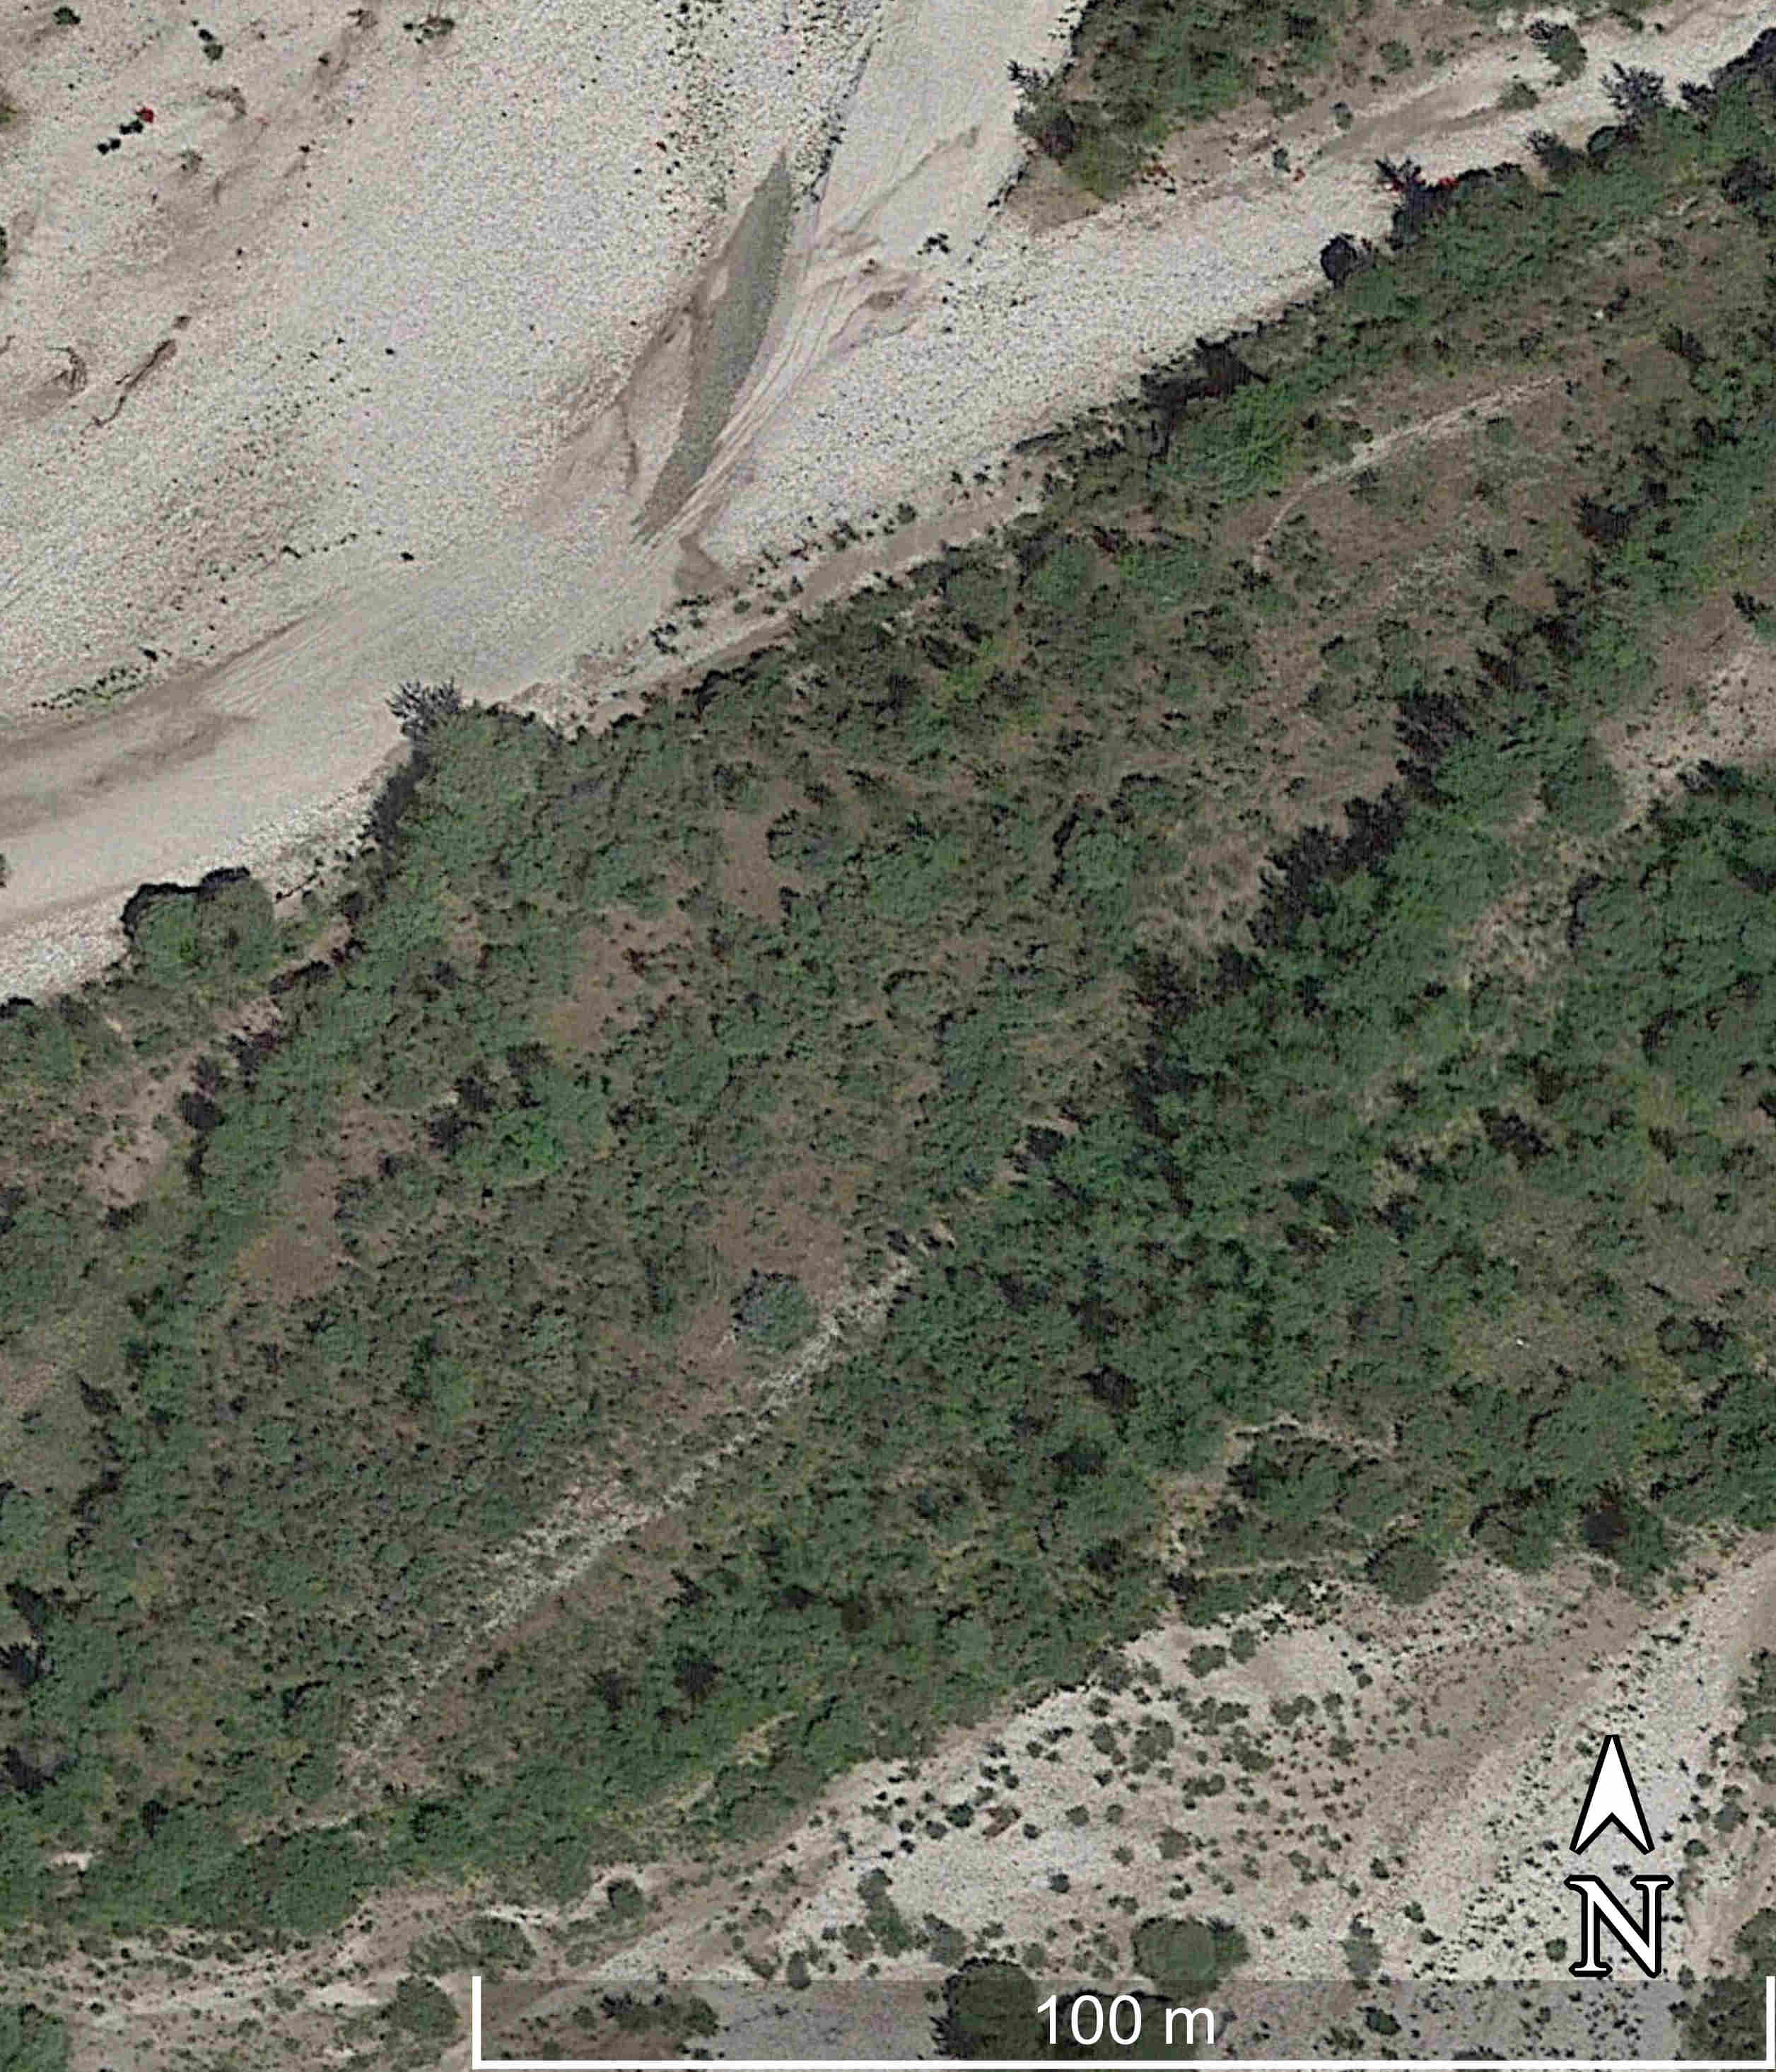
\includegraphics[width=\textwidth]{files/esempio_isola_sat_1.jpg}
		\caption{immagine da Google Earth di un isola in alveo.}
		\label{fig:esempio-isola-sat-1}
	\end{subfigure}
	\quad
	\begin{subfigure}[b]{0.57\textwidth}
		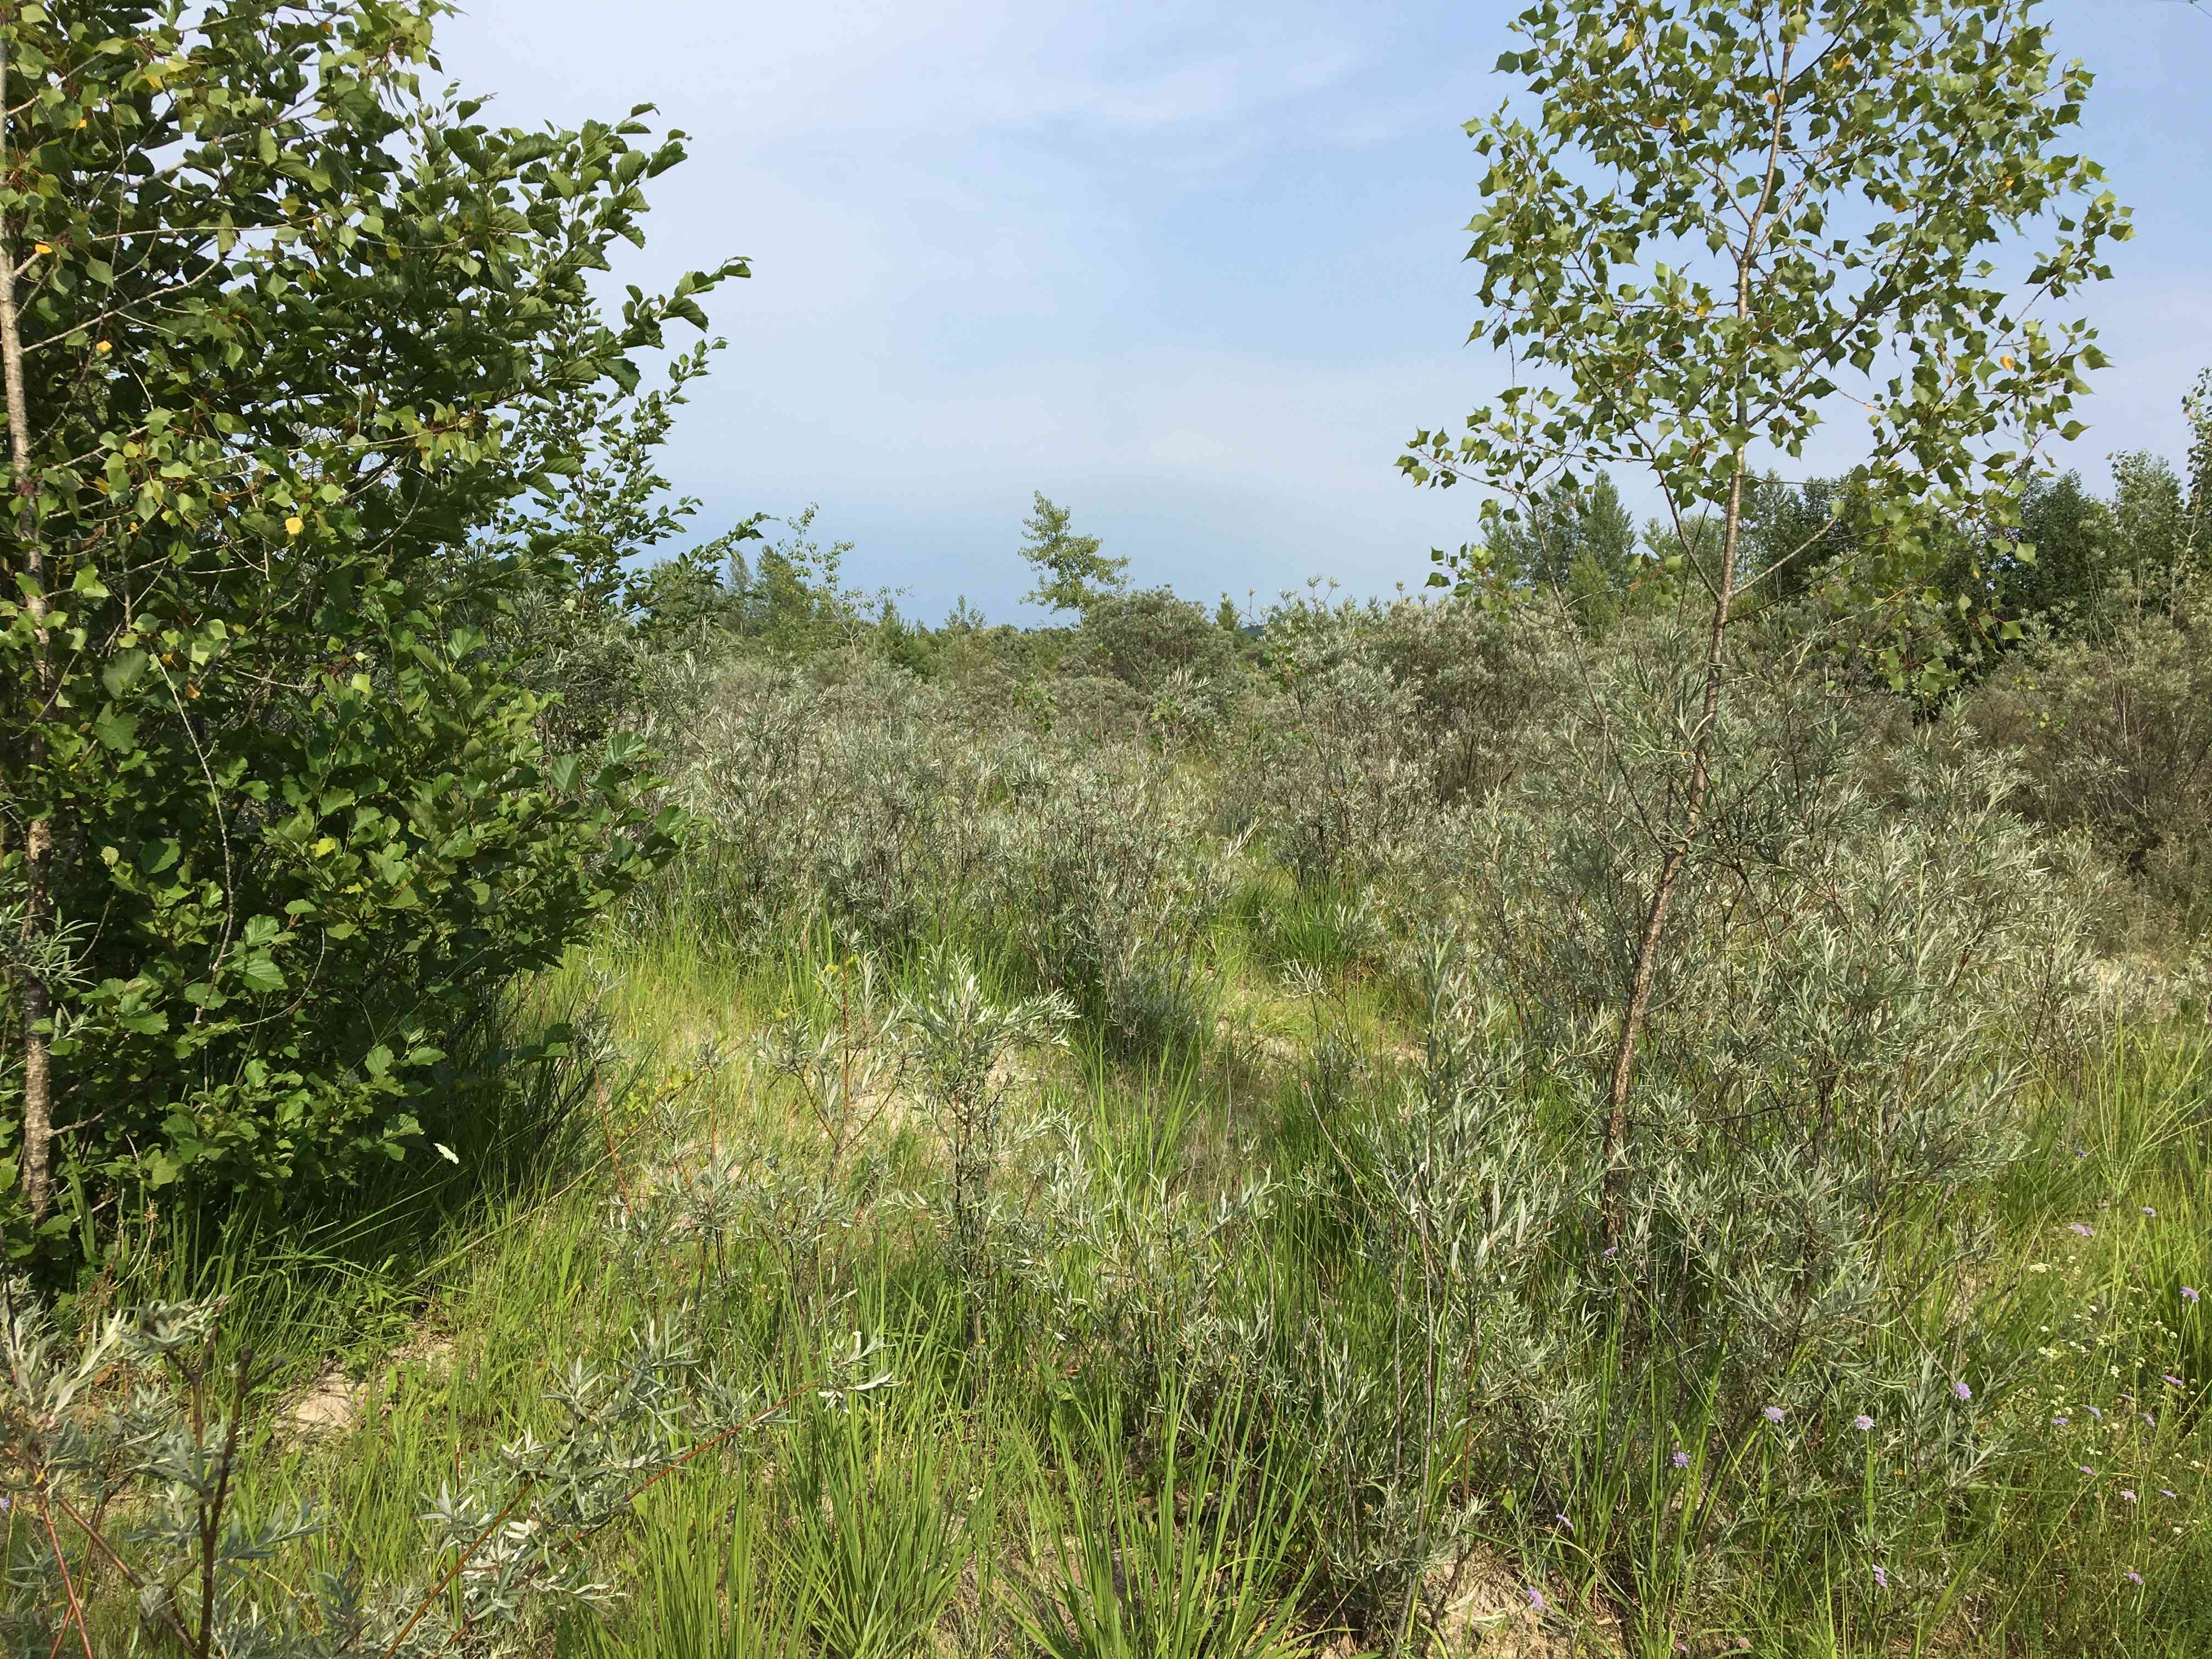
\includegraphics[width=\textwidth]{files/esempio_isola_1.jpg}
		\caption{foto di un isola molto vegetata presente nell'alveo del fiume.
		Foto dell'autore.}
		\label{fig:esempio-isola-1}
	\end{subfigure}
	\caption[immagine e foto di isole fluviali]{immagine e foto di isole fluviali; si noti la forte presenza di salici (\emph{Salix spp.}) e di pioppi (\emph{Populus spp.}); il luogo della foto è prossimo a quello dell'immagine.}
\end{figure}

\begin{figure}
	\centering
	\begin{subfigure}[b]{0.52\textwidth}
		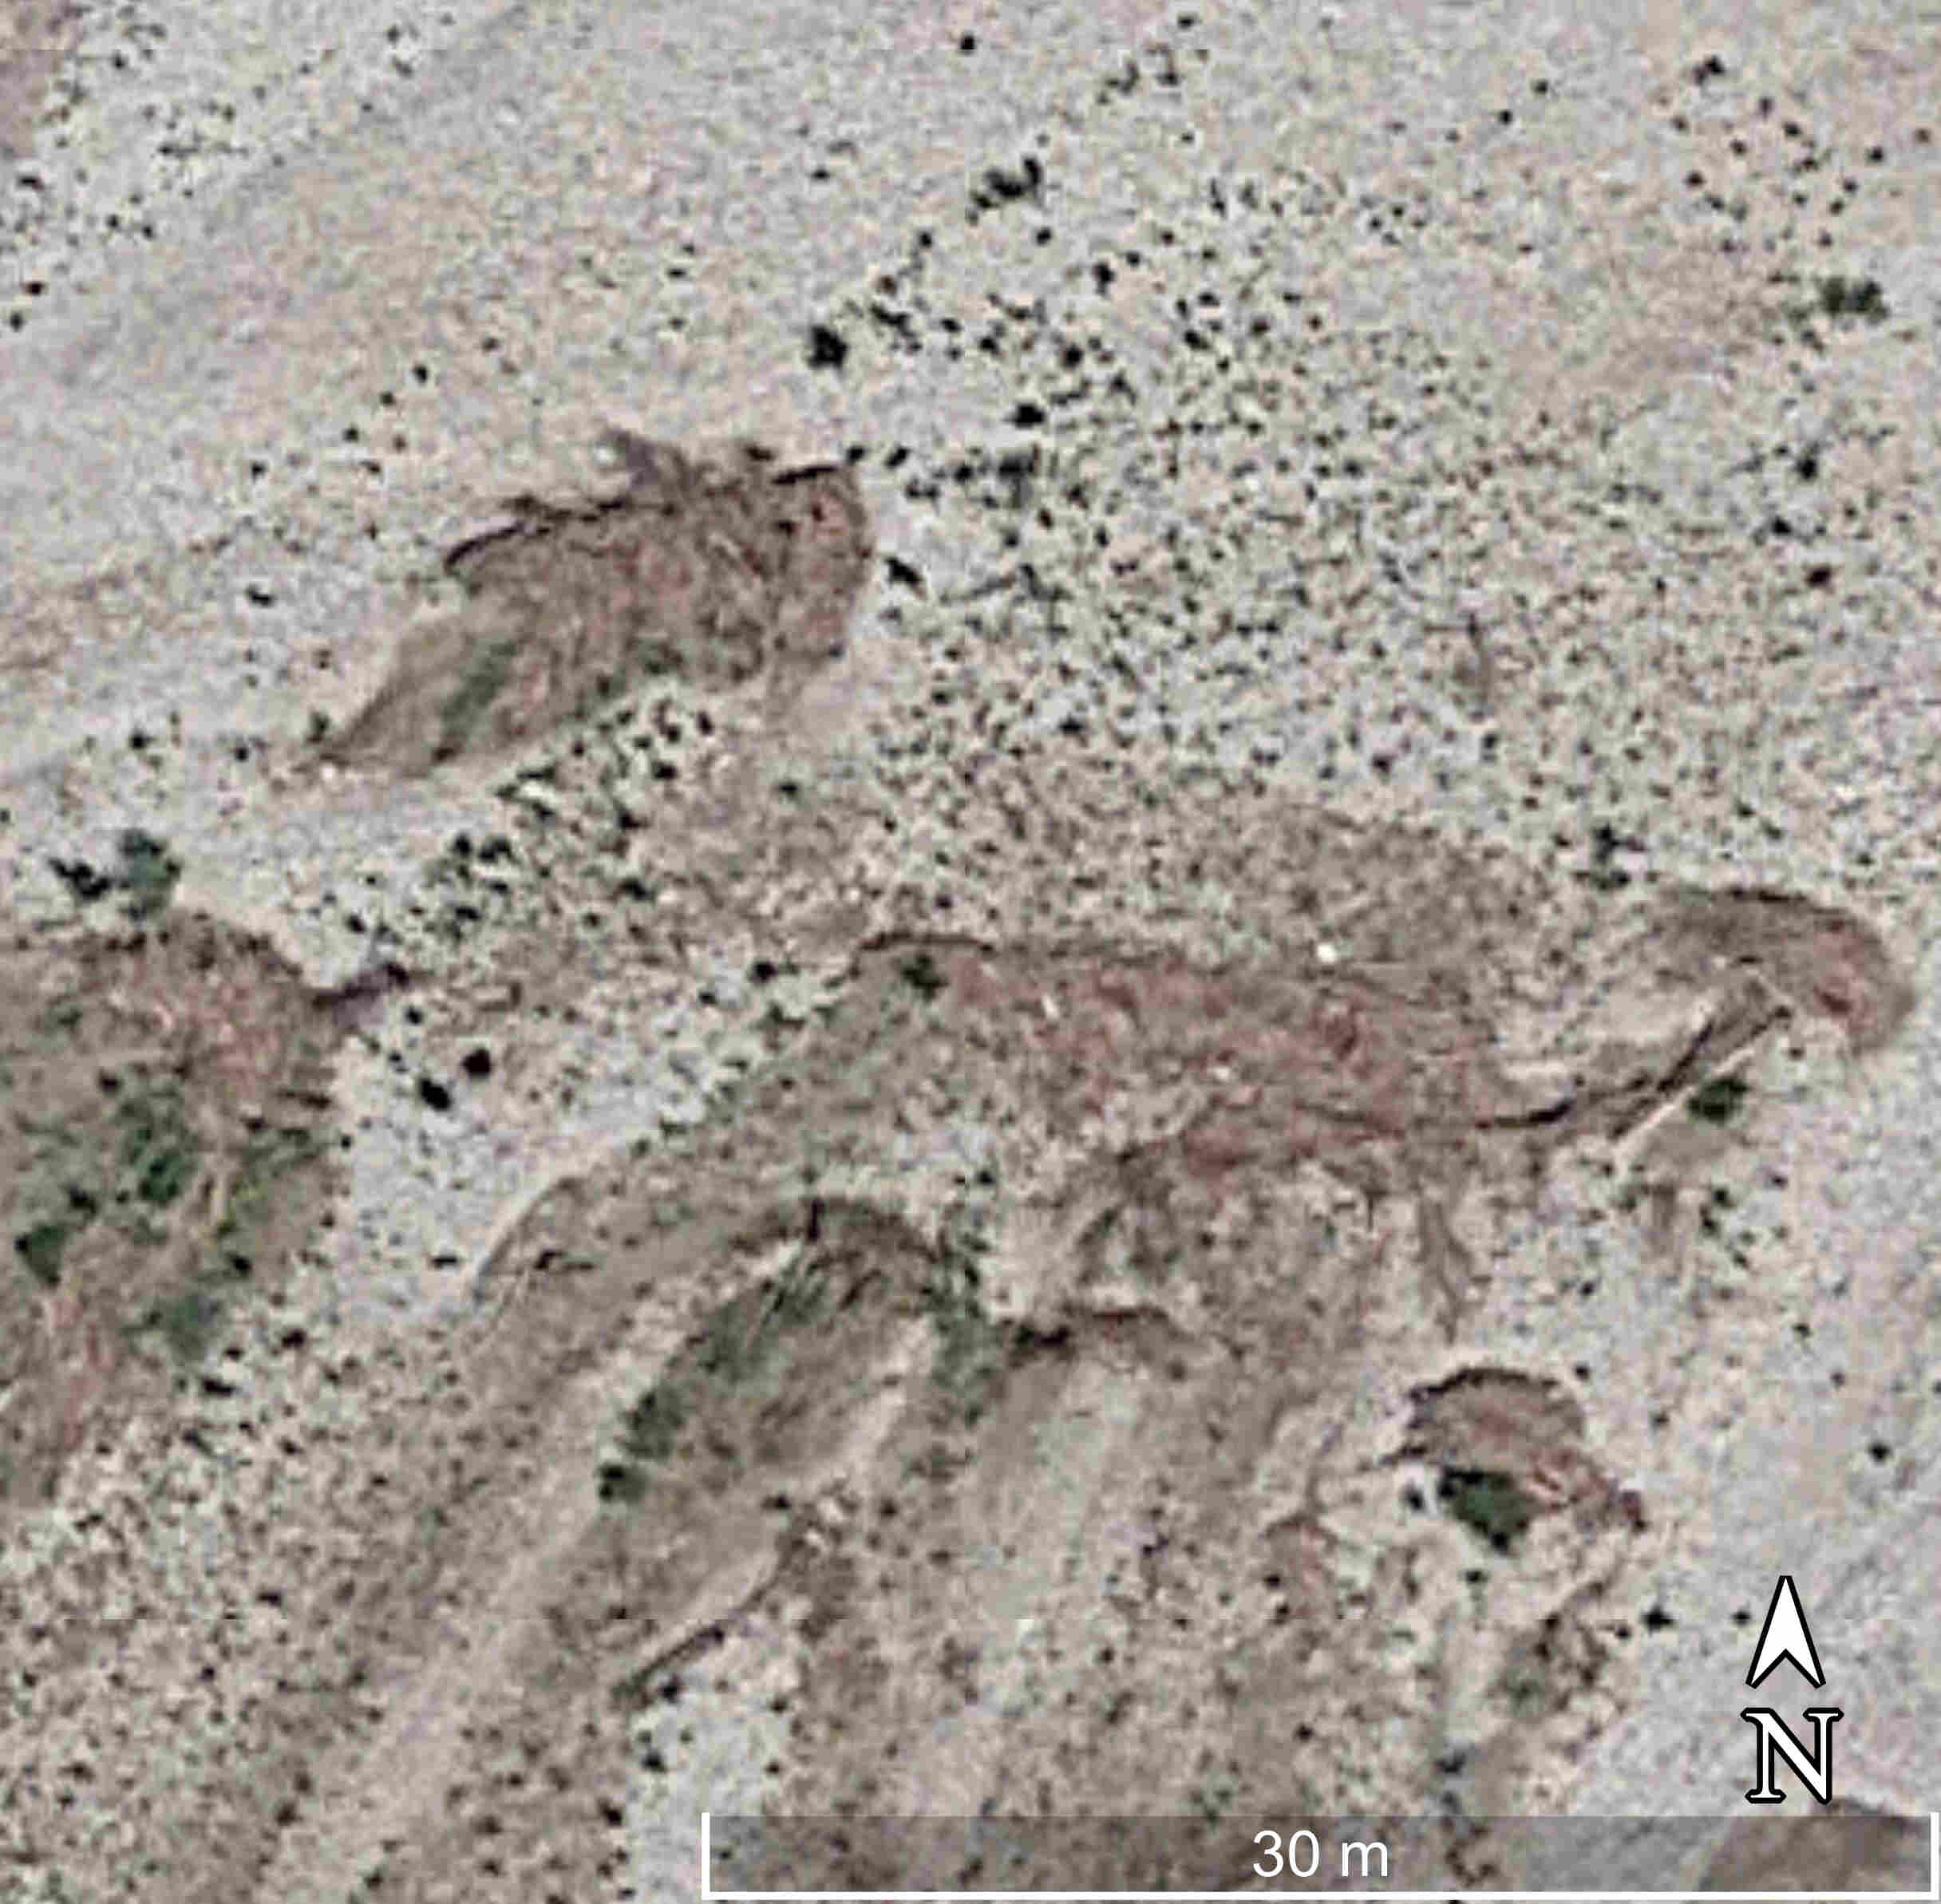
\includegraphics[width=\textwidth]{files/esempio_accumulo_sat_1.jpg}
		\caption{immagine da Google Earth di accumuli di legno e tronchi in alveo (in marrone chiaro).}
		\label{fig:esempio-accumulo-sat-1}
	\end{subfigure}
	\quad
	\begin{subfigure}[b]{0.44\textwidth}
		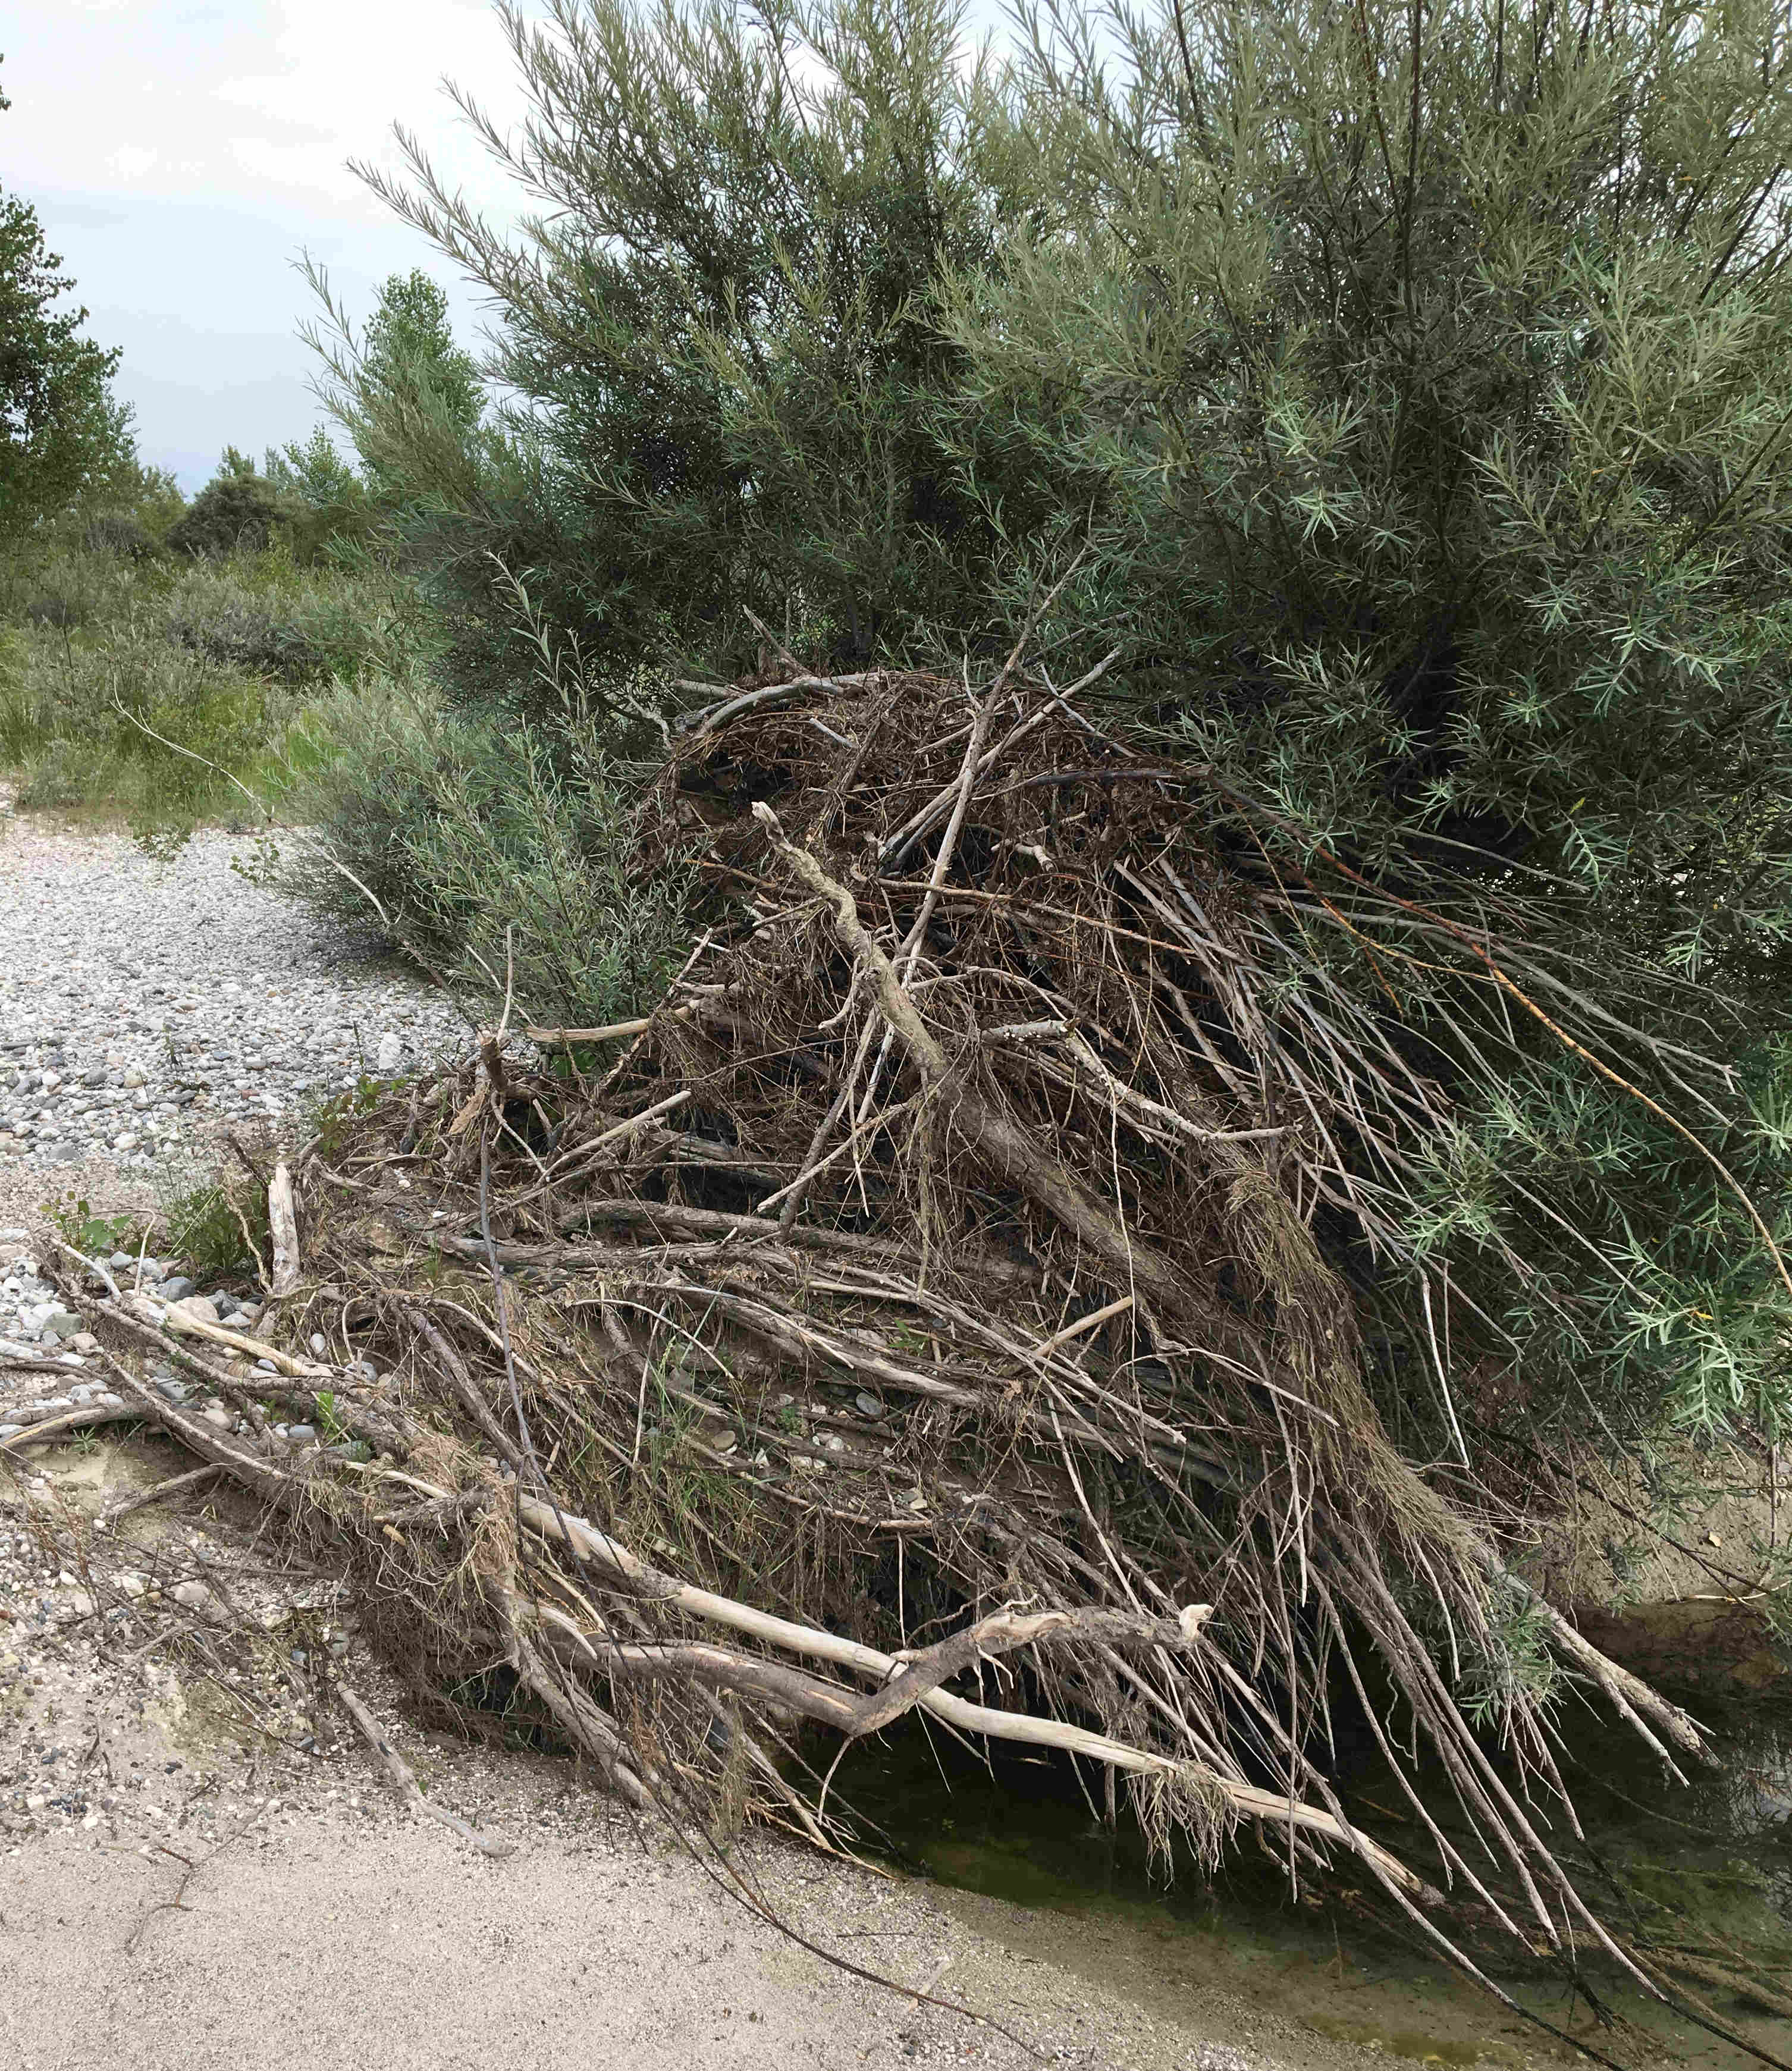
\includegraphics[width=\textwidth]{files/esempio_accumulo_1.jpg}
		\caption{foto di un accumulo di tronchi sopra una pianta di salice.
		Foto dell'autore.}
		\label{fig:esempio-accumulo-1}
	\end{subfigure}
	\caption[immagine e foto di accumuli legnosi]{immagine e foto di accumuli legnosi. Il luogo della foto non corrisponde a quello dell'immagine.}
\end{figure}


\section{Inquadramento dell'area di studio}
Il Fiume Tagliamento, situato nel Nord-Est italiano, è uno dei pochi fiumi alpini allo stato quasi naturale. 
Gli interventi effettuati sono arginature, derivazioni, pennelli, estrazione di ghiaia sia in tratti posti a monte che altri posti a valle; la loro entità è comunque tanto limitata da poter parlare di “contesto non gestito”.
\\
Il bacino idrografico del Tagliamento, ampio circa~\SI{2900}{\kilo\m\tothe{2}}, si estende tra le province di Udine, Pordenone e Venezia.
Il suo corso di circa~\SI{170}{\kilo\m} presenta morfologia intrecciata (\emph{braided}) nelle parti montane e planiziali con tratti larghi diverse centinaia di metri, se non più di \SI{1}{\kilo\m};
verso valle il fiume si restringe assumendo prima una forma transizionale monocursale con larghezza sui \SIrange[range-phrase={-}]{300}{200}{\m} nei pressi di Madrisio;
infine meandriforme a Latisana (larghezza intorno ai \SI{100}{\m}) fino alla foce, situata tra Bibione e Lignano.
\\
Insieme alla variazione della morfologia del fiume si assiste ad un cambiamento nella granulometria: mentre la ghiaia predomina nella parte intrecciata ($d_{50} = \SI{4}{\centi\m}$ \squarecites{Bertoldi:2010-d50}{Sitzia:2016-d50}), a partire dal tratto meandriforme si trova solo sabbia sul fondo.
Questo mutamento di materiale trasportato riflette la riduzione della pendenza che si osserva dal tratto transizionale monocursale e che giustifica il passaggio da fiume “in ghiaia” a fiume “in sabbia”.
\\
Il regime delle precipitazioni consiste di circa \SI{2000}{\mm} all'anno in media con forti variazioni locali; i minimi di precipitazione si registrano durante l'inverno, mentre i massimi in primavera e in autunno. Si assiste anche ad eventi di breve durata e particolarmente intensi.
Il regime fluviale che ne risulta è di tipo \emph{flashy} pluvio-nivale con piene brevi ed intense così come piene di diversi giorni di durata.

Il tratto studiato è quello intrecciato multicanale compreso tra Tolmezzo e Madrisio (\vref{fig:overview,fig:overview-sat}). 

In questo tratto nei pressi del paese di Pinzano è presente una stretta causata dall'affioramento di strati rocciosi che riduce la larghezza da diverse centinaia di metri a poco più di \SI{100}{\m}.
Questo restringimento assieme all'innalzamento dello strato di roccia che si trova sotto il letto del fiume induce l'acqua presente nella falda in alveo a risalire: si assiste al fenomeno dell'\emph{upwelling}. 
Similmente, a valle della stretta dove l'alveo non è più confinato e il letto roccioso sprofonda nel sottosuolo, l'acqua torna ad infiltrarsi nella ghiaia che forma il letto (\emph{downwelling}) fino a portare il fiume in condizioni di secca in certi tratti quando non ci sono piene.
\\
L'\emph{upwelling} e il \emph{downwelling} sono fenomeni rilevanti durante i periodi di magra: certi tratti a valle della stretta di Pinzano possono essere in condizioni di secca, privi completamente di acqua, la quale scorre tutta nel sottosuolo e riemerge quando la morfologia fluviale diventa transizionale vicino al ponte di Madrisio.
Durante le piene questi fenomeni sono invece irrilevanti: l'acqua che emerge o che si infiltra contribuisce minimamente alla portata fluente.

Nel tratto di studio vi sono diversi affluenti; vengono qui elencati da monte (Tolmezzo) fino a valle (Madrisio):
%
\begin{itemize}
	\item poco a valle di Tolmezzo c'è il Fella in sinistra idrografica (\SI{706}{\kilo\m\tothe{2}});
	\item all'altezza del paese di Venzone, in sinistra idrografica, sfocia il torrente Venzonassa (\SI{39}{\kilo\m\tothe{2}});
	\item qualche chilometro a monte del paese di Cornino in destra idrografica c'è il Leale (\SI{100}{\kilo\m\tothe{2}}), le cui acque riempiono i canali incisi del Tagliamento che in magra sono quasi secchi;
	\item in corrispondenza dell'isola di Cornino in sinistra idrografica il Ledra (\SI{75}{\kilo\m\tothe{2}}) riporta nel corso del Tagliamento le acque che si sono infiltrate nella piana di Osoppo;
	\item immediatamente a monte della stretta di Pinzano in destra idrografica si getta l'Arzino (\SI{123}{\kilo\m\tothe{2}});
	\item infine, una decina di chilometri più a valle della stretta in destra idrografica si incontra il Cosa (\SI{160}{\kilo\m\tothe{2}}).
\end{itemize}
%
Il contributo di questi affluenti in termini di portata non è trascurabile; tuttavia è raro che eventi di piena abbiano luogo contemporaneamente in tutti i sottobacini tanto da incrementare sensibilmente il livello d'acqua nel Tagliamento a valle degli affluenti durante una piena.
Si ritiene pertanto che conoscere il livello d'acqua in un punto del Tagliamento sia sufficientemente rappresentativo per descrivere l'entità di una piena in tutto il tratto di studio; inoltre si assume che la portata fluente sia proporzionale all'area drenante in ogni sezione del fiume.
%TODO immagine degli affluenti

%
\begin{figure}
	\centering
	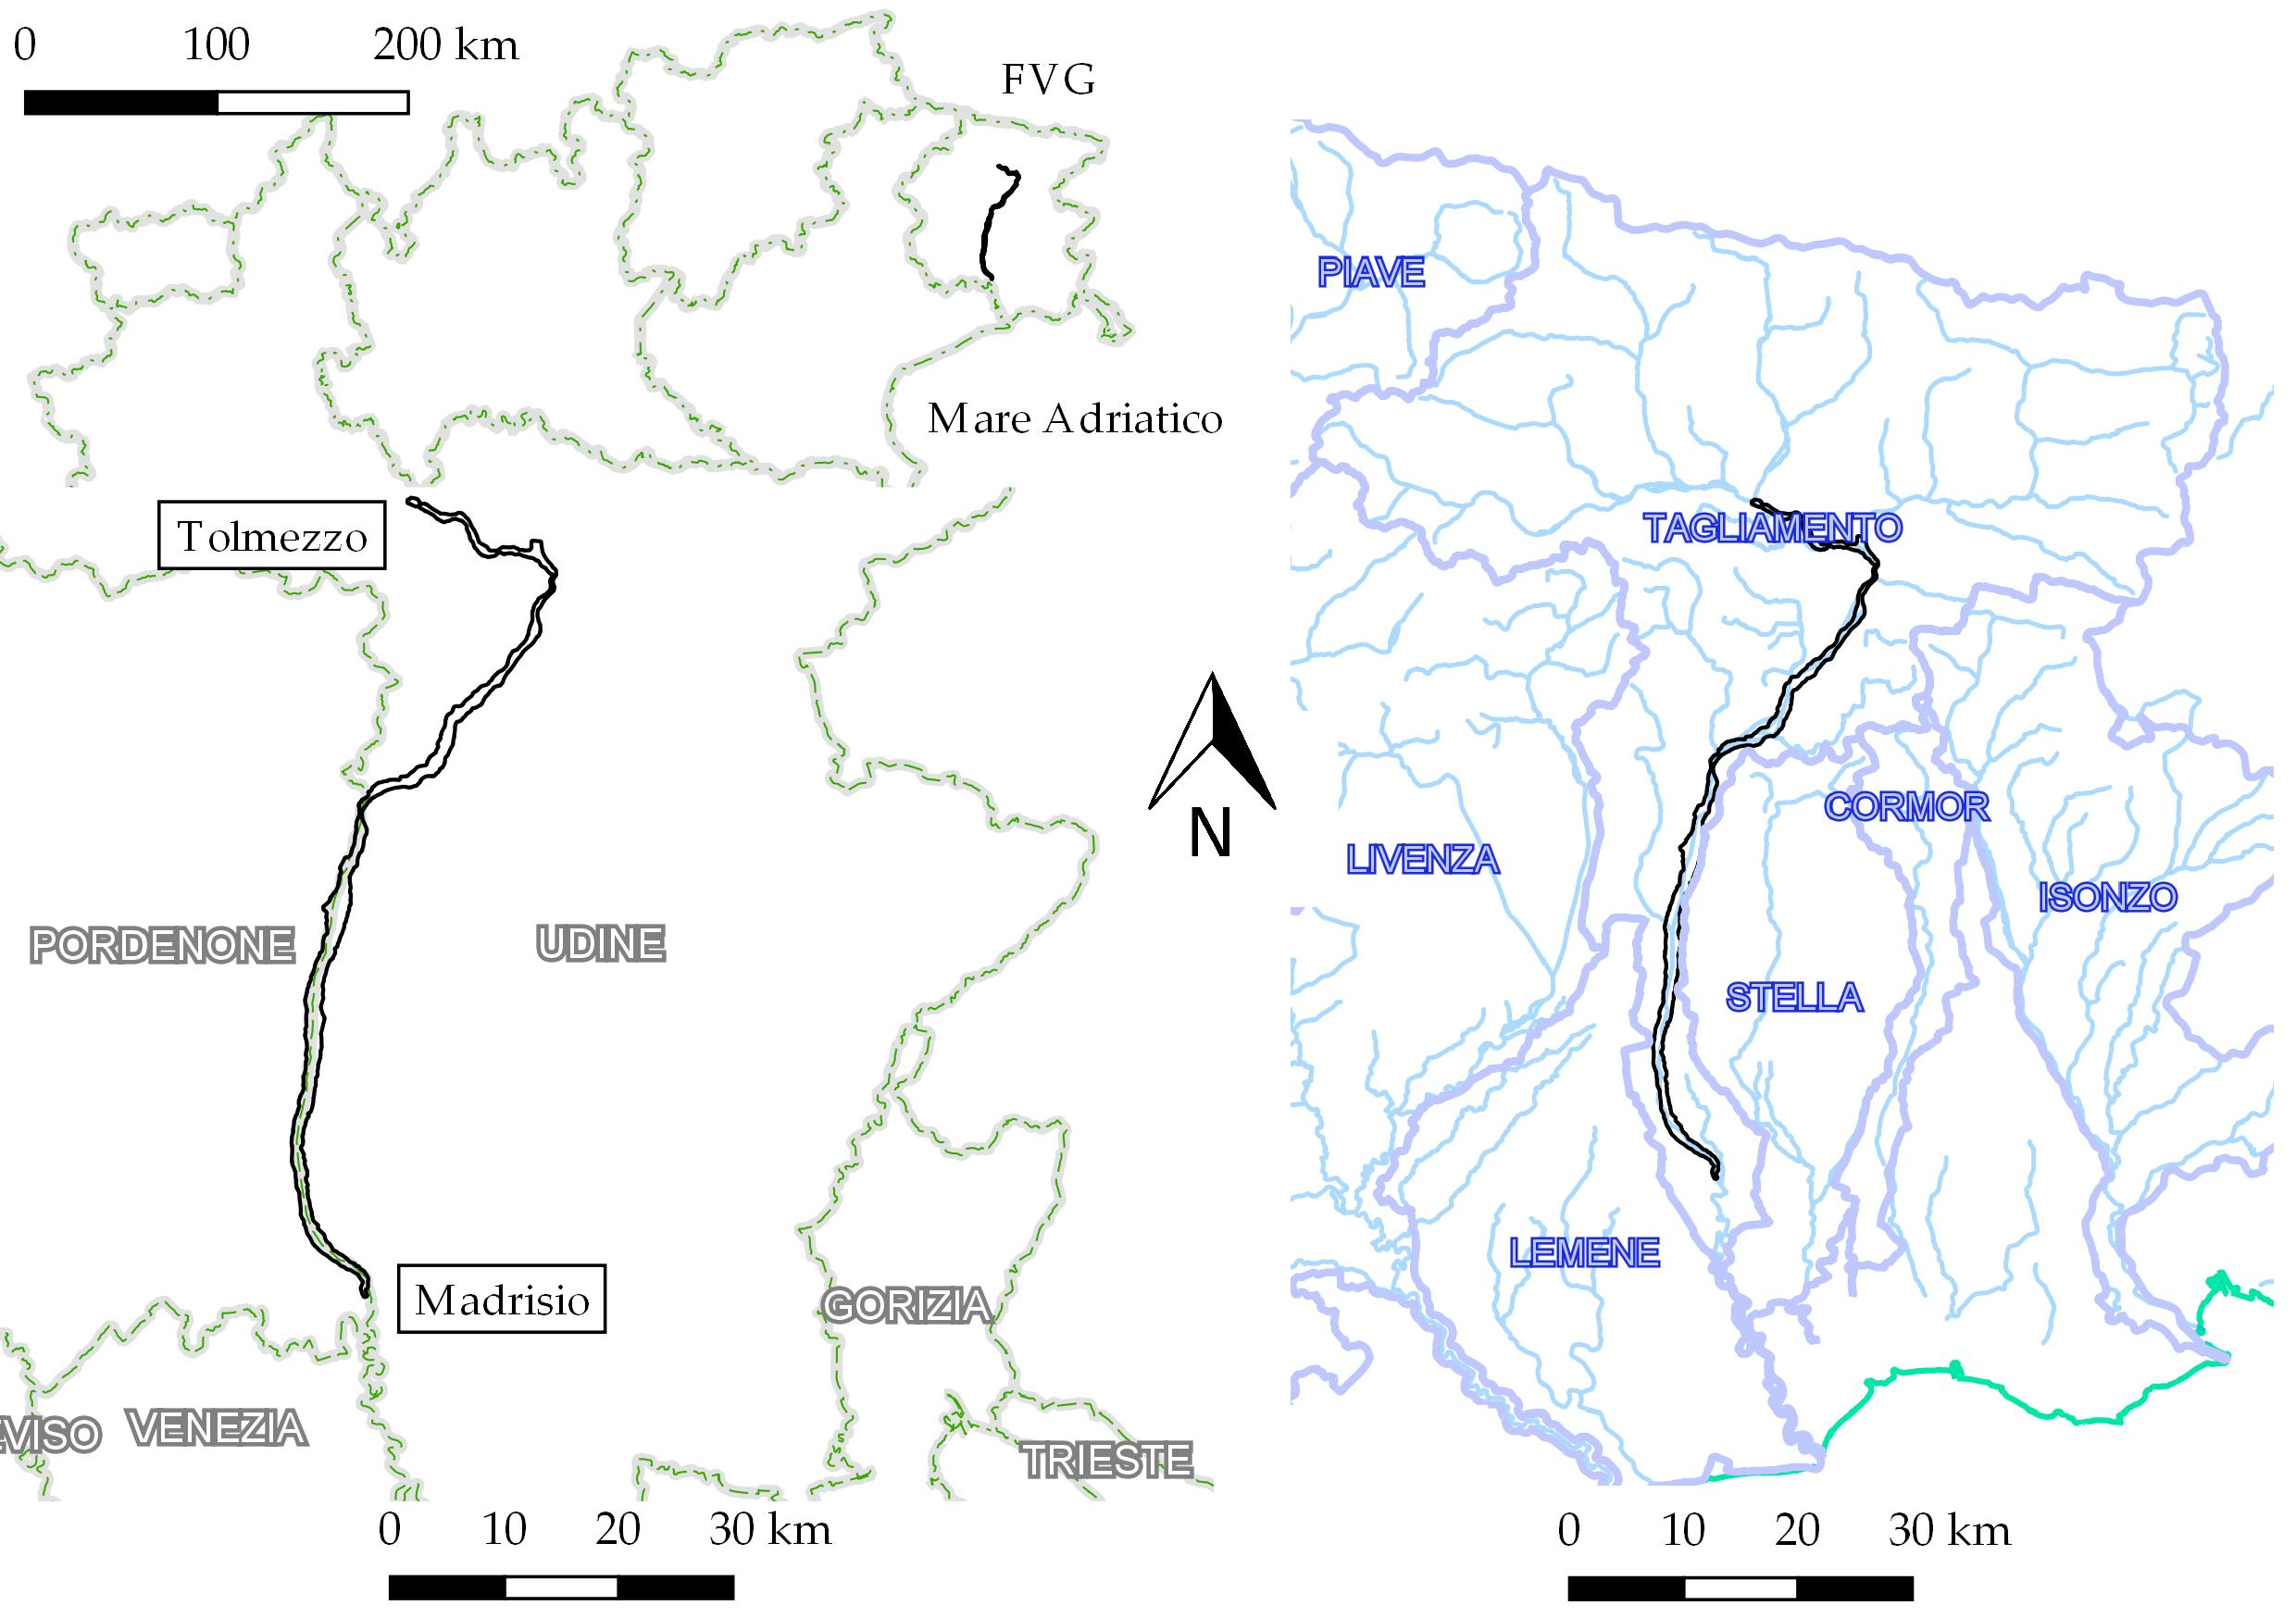
\includegraphics[width=\textwidth]{files/overview.jpeg}
	\caption[inquadramento dell'area di studio]
		{inquadramento dell'area di studio (poligono nero); a sinistra è mostrata l'Italia settentrionale (in alto) e un ingrandimento delle province e degli estremi dell'area di studio (in basso); a destra si vede il bacino idrografico del Tagliamento e di altri fiumi nelle vicinanze (in blu), il reticolo idrografico (in azzurro) e la linea di costa (in verde acqua).}
	\label{fig:overview}
\end{figure}
%
\begin{figure}
	\centering
	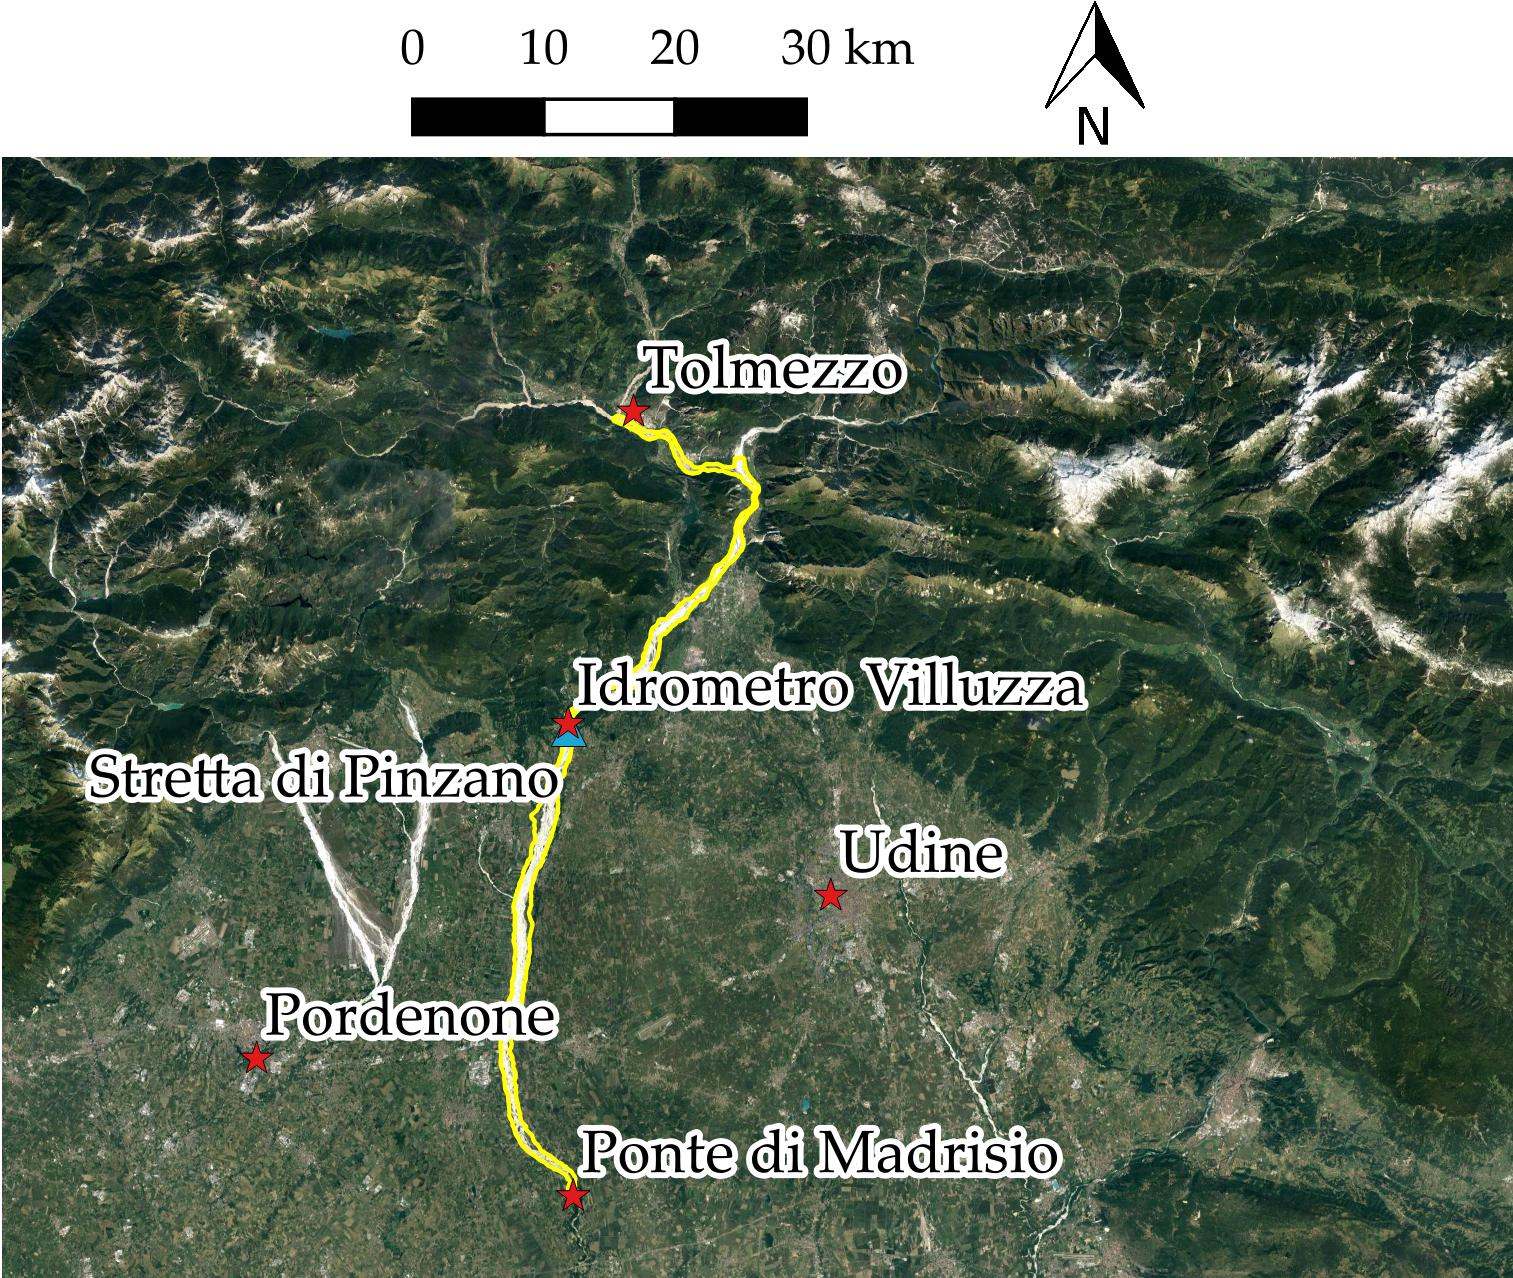
\includegraphics[width=\textwidth]{files/overview_tratto_sat.jpeg}
	\caption[inquadramento dell'area di studio]{inquadramento dell'area di studio (contornata in giallo).}
	\label{fig:overview-sat}
\end{figure}



\section{Stato dell'arte e valore aggiunto del presente lavoro}
In letteratura sono presenti numerosi lavori focalizzati su un tratto di circa~\SI{12}{\kilo\m} di lunghezza a monte della stretta di Pinzano; solitamente questi hanno utilizzato immagini ad alta risoluzione provenienti da voli aerei, le quali hanno una bassa risoluzione temporale (meno di una decina di immagini su un periodo di studio di diversi decenni).
\\
Le analisi svolte sono simili a quelle che questa tesi si propone di presentare: ricerca di una relazione tra isole erose e portata \squarecite{Surian:2015}, osservazione dell'evoluzione delle isole e della larghezza \squarecites{Surian:2015}{Bertoldi:2011-ASTER}{Zanoni:2008}.
\\
Le immagini satellitari \AST{} o LandSat~TM sono state utilizzate per gli scopi simili a quelli della presente tesi \squarecites{Bertoldi:2011-ASTER}{Henshaw:2013-LandSat}.
\\
Sono stati formulati diversi modelli concettuali sulle dinamiche vegetazionali nei fiumi, in particolare nel Tagliamento \squarecites{Gurnell:2001-island-formation}{Gurnell:2014-plants-eng}.

% i risultati di questi lavori attinenti al tema della tesi sono:
% a seguito di un progressivo restringimento esperito nella seconda metà del '900, nel primo decennio del 2000 il Tagliamento si è allargato

Il presente lavoro mira a :
\begin{itemize}
	\item utilizzare un maggior numero di immagini in un periodo di studio più breve, avvalendosi dei prodotti sia delle più recenti missioni spaziali sia di quelle relativamente più datate, e in un tratto di fiume più esteso; in tal maniera possono essere analizzati più fenomeni in maggior dettaglio;
	\item utilizzare ed estendere le metodologie, e di conseguenza anche i risultati, applicabili nello sfruttamento delle immagini satellitari;
	\item attraverso osservazioni e relazioni formalizzare modelli concettuali precedentemente elaborati;
	\item utilizzare dati provenienti da rilievi LiDAR per calcolare la \emph{stream power};
	\item ottenere delle relazioni più solide grazie alla maggior quantità di dati disponibili;
	\item aggiungere nuove osservazioni a quelle effettuate in precedenza;
	\item mostrare che è possibile effettuare un monitoraggio delle dinamiche fluviali quasi in tempo reale. 
\end{itemize}



\section{Convenzioni}
Le seguenti convenzioni saranno utilizzate nella presente tesi:
\begin{description}
	\item[Mappe] riportate secondo WGS84/UTM~33N (EPSG:~32633);
	\item[Direzione della corrente] riportata con una freccia blu nelle immagini;
	\item[Formato delle date] AAAA-MM-GG;
	\item[Citazioni] sono nel formato Autore/i-Anno, racchiuse tra parentesi quadre;
	\item[Web link] sono riportati in note a piè pagina;
	\item[Termini in lingua straniera] sono in corsivo;
	\item[Glossario] presente nel materiale finale.
	%
\end{description}




\section{Lo strumento principale: la radiazione elettromagnetica}
Gli strumenti di acquisizione di immagini aeree e satellitari sono sensibili a determinate lunghezze d'onda della radiazione elettromagnetica (\vref{graph:el-mag-radiation}), cioè sono in grado di registrarne solo alcune porzioni (bande).
L'occhio umano può distinguere solo le bande del visibile, mentre i sensori artificiali possono acquisire altre bande della radiazione.
%
\begin{figure}
	\centering
	\tikzsetnextfilename{electromagnetic_radiation}
\begin{tikzpicture}[fill between/on layer={axis grid}]
	\begin{axis}[
		xlabel={Lunghezza d'onda},
		xticklabel style = {font=\tiny,yshift=0.2ex},
		xmin=10^-5,
		xmax=10^9,
		x unit=\si{\micro\meter},
		xmode=log,
		ymin=0,
		ymax=1,
		height=3cm,
		width=\textwidth,%12.2cm,
		yticklabels={},
		ytick=\empty,
		legend cell align=left,
		legend style={
			at={(0.5,-0.8)},%(0.85,-0.77)},
			anchor=north,
			legend columns=4,
			}
	]
	\addplot[draw=none, name path=start, forget plot] coordinates{(10^-5,0)(10^-5,1)};
	\addplot[draw=none, name path=gamma, forget plot] coordinates{(10^-3,0)(10^-3,1)};
	\addplot[draw=none, name path=xrays, forget plot] coordinates{(10^-2,0)(10^-2,1)};
	\addplot[draw=none, name path=uv, forget plot] coordinates{(0.4,0)(0.4,1)};
	\addplot[draw=none, name path=visible, forget plot] coordinates{(0.7,0)(0.7,1)};
	\addplot[draw=none, name path=ir, forget plot] coordinates{(10^2.5,0)(10^2.5,1)};
	\addplot[draw=none, name path=microwave, forget plot] coordinates{(10^5,0)(10^5,1)};
	\addplot[draw=none, name path=radiowave, forget plot] coordinates{(10^9,0)(10^9,1)};
	\addplot[violet!20, area legend] fill between[of=start and gamma];
	\addlegendentry{Raggi $\gamma$}
	\addplot[violet!60, area legend] fill between[of=gamma and xrays];
	\addlegendentry{Raggi X}
	\addplot[violet, area legend] fill between[of=xrays and uv];
	\addlegendentry{Ultravioletti}
	\addplot[shading=visiblelight, area legend] fill between[of=uv and visible];
	\addlegendentry{Luce visibile}
	\addplot[red, area legend] fill between[of=visible and ir];
	\addlegendentry{Infrarosso}
	\addplot[Bittersweet, area legend] fill between[of=ir and microwave];
	\addlegendentry{Microonde}
	\addplot[Brown, area legend] fill between[of=microwave and radiowave];
	\addlegendentry{Onde radio}
	\end{axis}
\end{tikzpicture}

	\caption{radiazione elettromagnetica con le sue lunghezze d'onda.}
	\label{graph:el-mag-radiation}
\end{figure}
%
\\
Le immagini nel visibile sono solitamente suddivise nelle bande del Rosso, Verde e Blu (\emph{Red}, \emph{Green}, \emph{Blue}, R-G-B); ognuna indica la quantità di colore presente; la combinazione di queste quantità di colore restituisce l'immagine a colori.
\\
Per poter osservare immagini con bande diverse dal visibile si sostituisce una o più bande R-G-B con le bande in questione.
Ad esempio, è possibile sostituire la banda del Rosso con quella dell'Infrarosso (IR): la quantità di colore del Rosso sarà rimpiazzata dalla quantità di colore dell'Infrarosso.
Il risultato sarà un'immagine riconoscibile dall'occhio umano, ma in falsi colori (\vref{fig:confronto-bande-intro}).
%
\begin{figure}
	\centering
	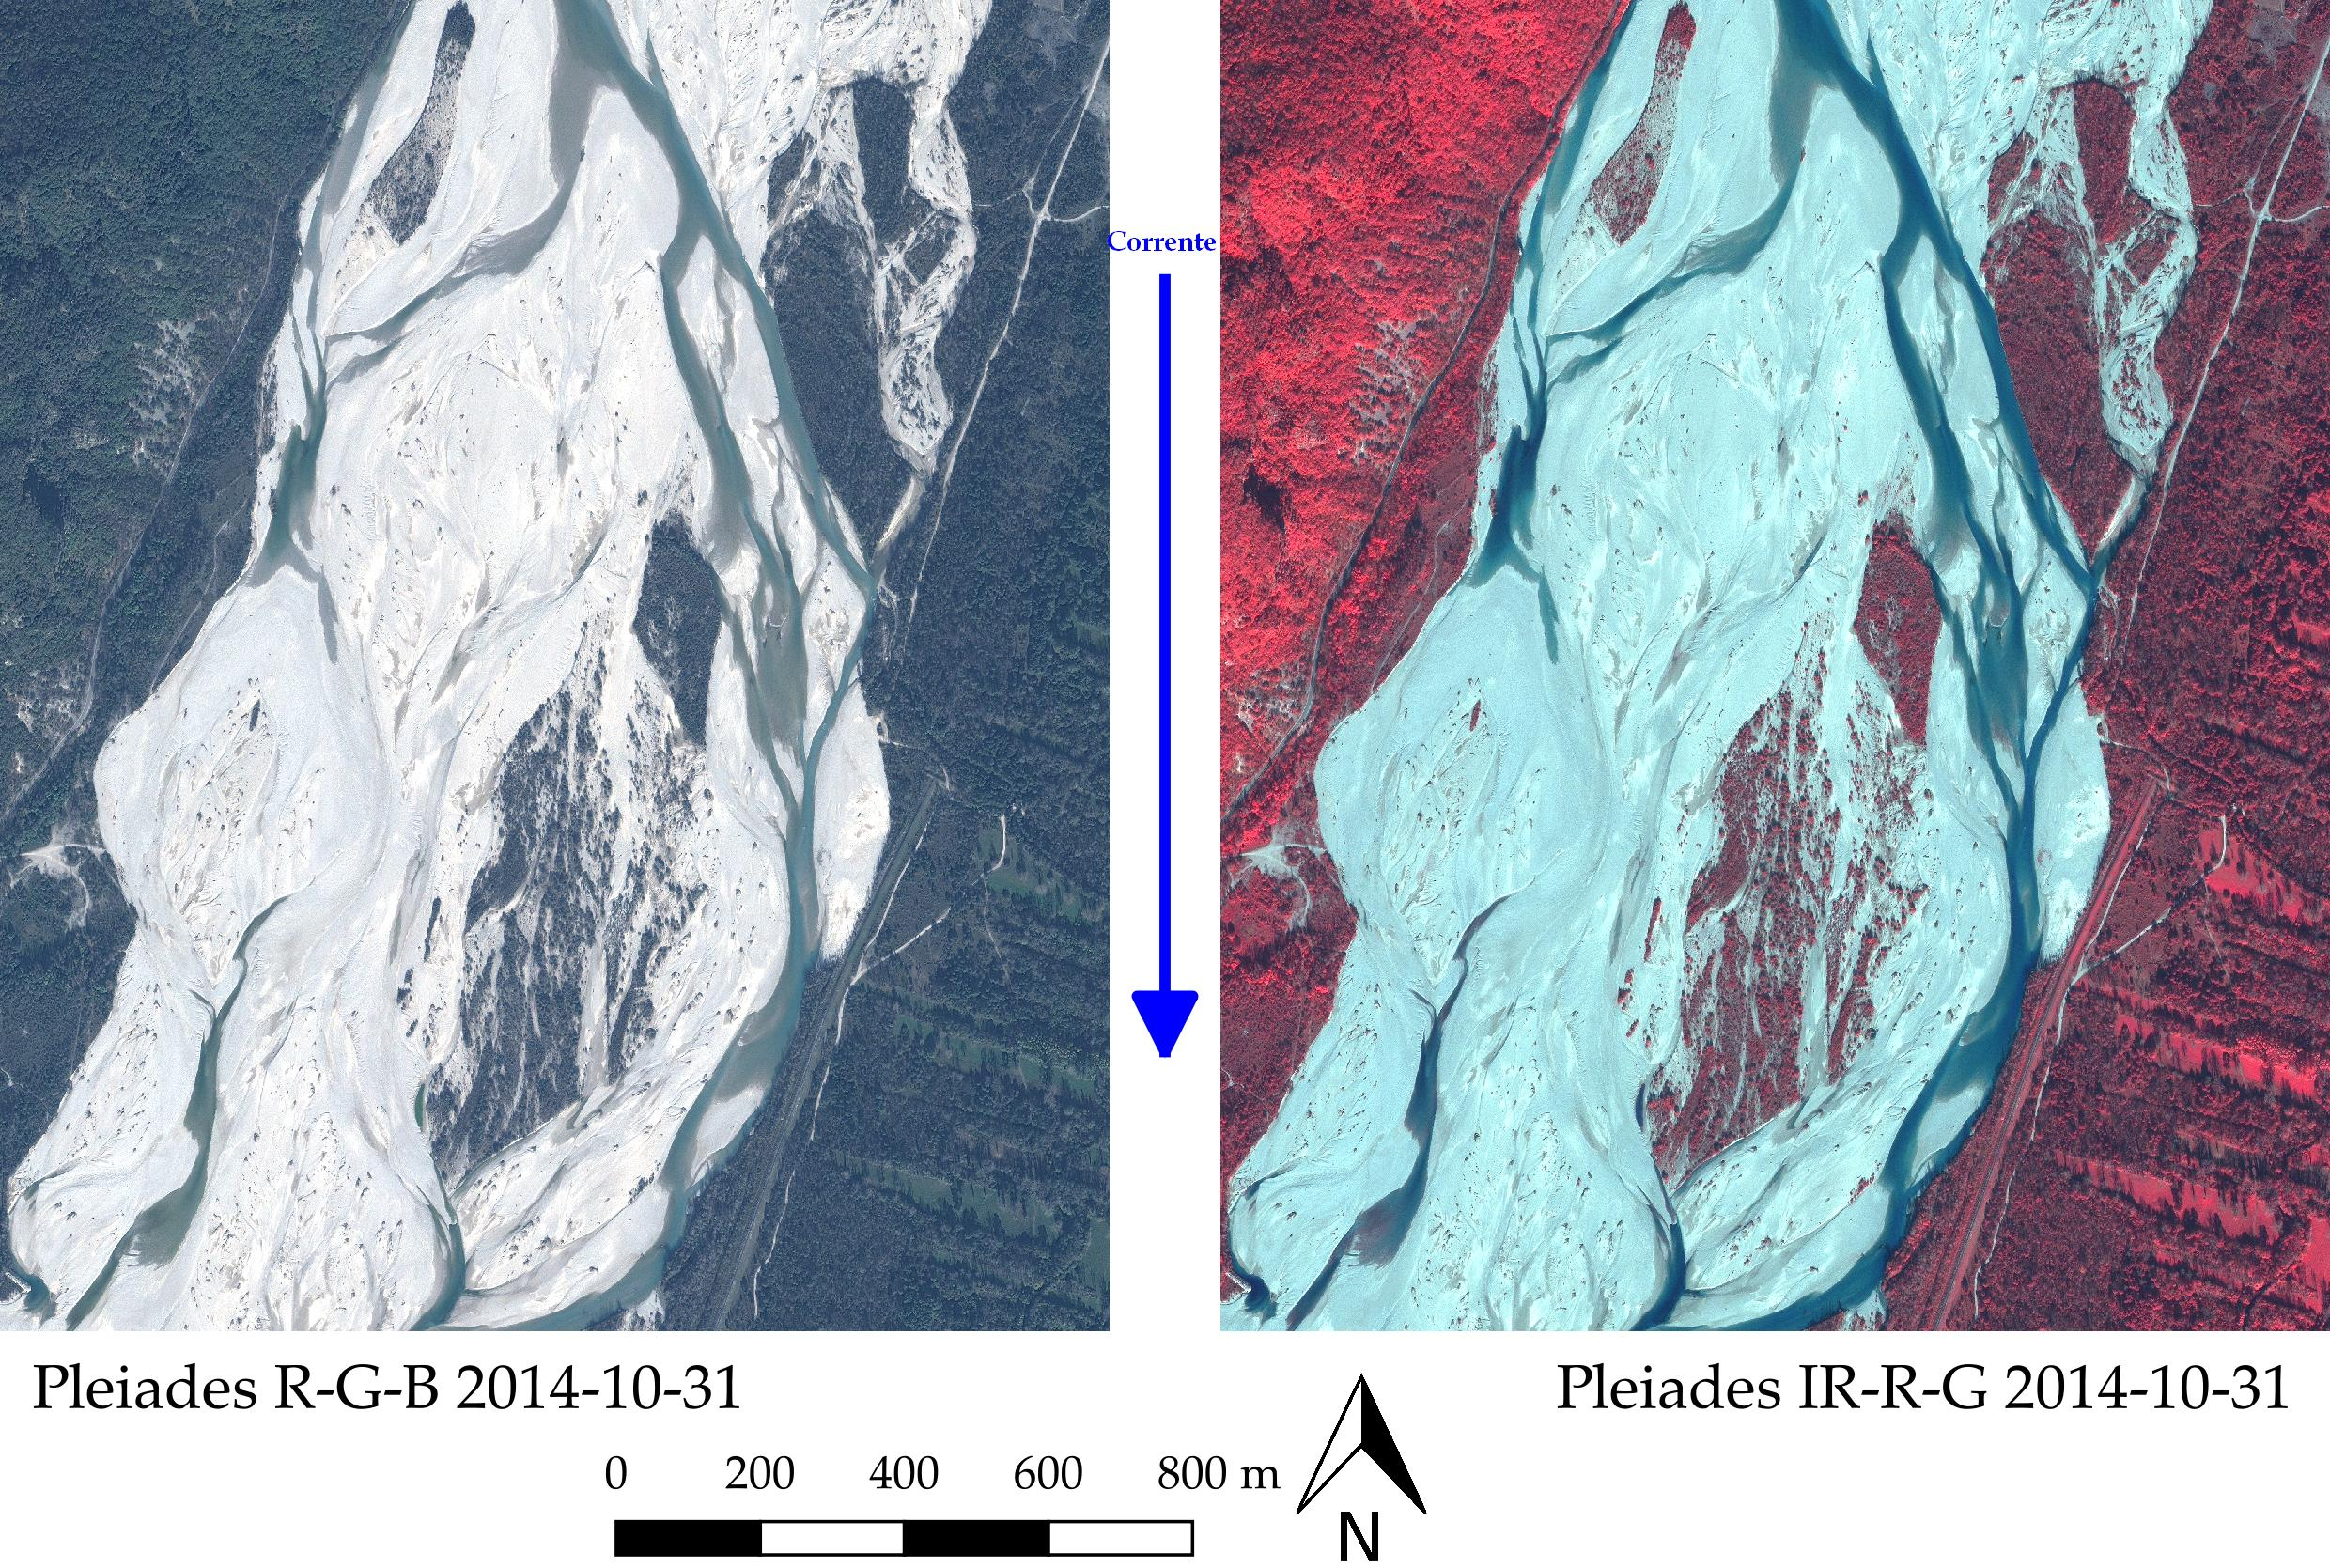
\includegraphics[width=\textwidth]{files/confronto_bande_intro.jpeg}
	\caption[confronto immagini R-G-B e IR-R-G]{confronto di un'immagine in veri colori (R-G-B, a sinistra) con una in falsi colori (IR-G-B, a destra); quest'ultima evidenza la presenza di vegetazione viva rispetto alla ghiaia in alveo e all'acqua nei canali.}
	\label{fig:confronto-bande-intro}
\end{figure}
%
\\
Questo procedimento serve per distinguere più facilmente degli elementi e degli oggetti presenti nelle immagini; per esempio la vegetazione viva riflette particolarmente la banda dell'Infrarosso più vicina al Rosso.



\section{Materiali}
% materiali
\paragraph{Immagini aeree e satellitari}
Sono state considerate le bande del \emph{Near-InfraRed}~(NIR) e del \emph{Red}~(R) nelle immagini satellitari multibande provenienti dalle seguenti missioni:
%
\begin{itemize}
	\item satellite Terra, sensore \AST{} Livello~1T (ottenuti in data~21~luglio~2018 e~30~settembre~2018 \squarecite{data:ASTER});  
		\\
		NIR (Banda~3N)~\SIrange[range-phrase={-}]{0.78}{0.86}{\nano\m}, R (Banda~2)~\SIrange[range-phrase={-}]{0.63}{0.69}{\micro\m};
	\item costellazione \Pl{} (\href{https://pleiades.cnes.fr/en/PLEIADES/index.htm}{Centre National d'Etudes Spatiales}\footnote{\texttt{https://pleiades.cnes.fr/en/PLEIADES/index.htm}}), immagini acquistate dall'Università degli Studi di Trento; 
		\\
		NIR~\SIrange[range-phrase={-}]{0.74}{0.94}{\micro\m}, R~\SIrange[range-phrase={-}]{0.59}{0.71}{\micro\m};
	\item satellite \Se{}A-B, sensore~MSI Livello~1C (ottenuti in data 21~luglio 2018 e~21~novembre~2018 tramite il \href{http://scihub.copernicus.eu/}{Copernicus Open Access Hub}\footnote{\texttt{http://scihub.copernicus.eu/}});
		\\
		NIR (Banda~8)~\SIrange[range-phrase={-}]{0.763}{0.908}{\micro\m}, R (Banda~4)~\SIrange[range-phrase={-}]{0.645}{0.683}{\micro\m};
	\item satellite \WV{} (\href{satimagingcorp.s3.amazonaws.com/site/pdf/WV1\_{}WV2\_{}SpectralResponse.pdf}{DigitalGlobe}\footnote{\texttt{satimagingcorp.s3.amazonaws.com/site/pdf/WV1\_{}WV2\_{}SpectralResponse.pdf}}), immagini acquistate dall'Università degli Studi di Trento;
		\\
		NIR (Banda~MS1)~\SIrange[range-phrase={-}]{0.770}{0.895}{\micro\m}, R (Banda~MS2)~\SIrange[range-phrase={-}]{0.630}{0.690}{\micro\m}.
\end{itemize}
%

Le ortofoto dell'estate~2011 provengono dal \href{http://www.pcn.minambiente.it/mattm/}{Portale Cartografico Nazionale del Ministero dell'Ambiente e della tutela del territorio e del mare}\footnote{\texttt{http://www.pcn.minambiente.it/mattm/}};
le ortofoto del~2013 sono state ottenute da volo \href{http://www.cgrspa.com/}{CGR}\footnote{\texttt{http://www.cgrspa.com/}} su commissione; 
le ortofoto del~2017 sono state ottenute da \href{https://www.google.com/earth/}{Google Earth}\footnote{\texttt{https://www.google.com/earth/}}.

Assieme alla ortofoto del~2013 è stato effettuato un rilievo LiDAR, grazie al quale sono a disposizione un DEM (\emph{Digital Elevation Model}) e un CSM (\emph{Canopy Surface Model}): il primo consiste di una mappa con le quote del suolo; il secondo è una mappa di altezza della vegetazione.

Il DEM del~2009 proviene dal \href{http://irdat.regione.fvg.it/CTRN/ricerca-cartografia/}{Portale Cartografico della regione autonoma Friuli Venezia Giulia}\footnote{\texttt{http://irdat.regione.fvg.it/CTRN/ricerca-cartografia/}}.

È bene evidenziare che le mappe non hanno tutte la medesima estensione e una piccola parte non comprende tutto il tratto oggetto di studio.
Ciò limita minimamente le analisi che è possibile fare.
\\
La risoluzione temporale, inferiore ad~\SI{1}{\anno} con \num{25} immagini per un periodo di studio di quasi \SI{19}{\anni}, è sufficiente per interpretare i processi che hanno luogo nel Tagliamento; la risoluzione spaziale varia da~\SIrange[range-phrase={ a }]{15}{0.5}{\m}, adeguata per poter distinguere correttamente le caratteristiche del fiume (limite dell'alveo attivo, isole, canali nella \emph{floodplain}, canali attivi, \ldots).

\paragraph{Dati idrometrici}
I dati idrometrici orari o semi-orari dal 2000-01-01 al 2018-10-14 presso l'idrometro di Villuzza (\SI{46.181}{\degree}N, \SI{12.958}{\degree}E, quota~\SI{240}{\m}~s.l.m.m., corrispondente al ponte di Pinzano) sono stati forniti dalla \href{http://www.protezionecivile.fvg.it/it/rete-idrometeorologica}{rete idrometeorologica della Protezione Civile della Regione Autonoma Friuli Venezia Giulia}\footnote{\texttt{http://www.protezionecivile.fvg.it/it/rete-idrometeorologica}}.
Questi dati consistono dell'altezza del pelo libero dell'acqua rispetto ad un livello di riferimento locale dell'idrometro.
La dinamica della morfologia del fondo del fiume non permette di ottenere una scala di deflusso (delle portate) generalmente valida; ciò comunque non costituisce un limite.

I grafici in \vref{graph:livelli-orto-sat} mostrano rispettivamente la media giornaliera dei livelli idrometrici e le date di cui si dispongono ortofoto e immagini satellitari (\AST{}, \Pl{}, \Se{}, Google~Earth, \WV{}). 
Nel secondo grafico sono riportati solamente i livelli medi giornalieri maggiori di~\SI{2}{\m} in quanto livelli superiori a tale soglia iniziano ad avere effetti di disturbo sulla vegetazione \squarecite{Bertoldi:2009-2m}.
La \vref{tab:date-orto-sat} mostra le date e la dimensione delle celle delle immagini utilizzate nell'analisi.
%%
\begin{figure}[p]
	\centering
	\begin{tikzpicture}
	%\begin{groupplot}
	\begin{axis}[
		%name = orto-sat,
		axis y line* = right,
		axis x line* = top,
		%height = .3\textwidth,
		width = \textwidth,
		date coordinates in = x,
		%symbolic y coords = {ASTER,PLEIADES,SENTINEL2,G-EARTH},
		xticklabel = {\year-\month-\day},
		xtick = data,
		ytick = data,
		xticklabel style = {
			rotate = 90,
			anchor = near xticklabel
		},
		enlarge x limits = 0.05,
		enlarge y limits = 0.01,
		ylabel = {Fonte},
		ymax = 3.6,
		ymin = -0.1,
		grid = none,
		only marks,
		]
		\addplot table [x=data, y=numero] {graphics/data/data-orto-sat.txt};
	\end{axis}
	%
	\begin{axis}[
		%name = stages,
		%at = {($(orto-sat.south)-(0,2cm)$)},
		%anchor = north,
		axis y line* = left,
		width = \textwidth,
		date coordinates in = x,
		xticklabel = {\year-\month-\day},
		xticklabel style = {
			rotate = 45,
			anchor = near xticklabel
		},
		enlarge x limits = 0.05,
		enlarge y limits = 0.01,
		ymax = 3.6,
		ymin = -0.1,
		ylabel = {Livello idrometrico},
		grid = major,
		no markers,
		]
		\addplot table [x=data, y=media-gg] {graphics/data/Dati_Villuzza.csv};
	\end{axis}
\end{tikzpicture}
	\tikzsetnextfilename{livelli_2m+imm}
\begin{tikzpicture}
	\begin{axis}[
		width = \textwidth,
		height = 0.5\textwidth,
		date coordinates in = x,
		date ZERO = 2000-01-01,
		xticklabel = {$\year$},
		xticklabel style = {
			rotate = 80,
			anchor = near xticklabel
		},
		xtick distance = 732,
		enlarge x limits = 0.05,
		enlarge y limits = 0.01,
		ymax = 3.7,
		ymin = 1.95,
		ylabel = {Livello idrometrico \si{[\m]}},
		grid = major,
		]
		\addplot+ 
			[red, mark=x, semithick, style=solid, mark=x]
			coordinates {(2000-09-17, 2)(2000-09-17, 3.7)};
		\addplot+ 
			[red, semithick, style=solid, mark=x]
			coordinates {(2001-06-07, 2)(2001-06-07, 3.7)};
		\addplot+
        	[red, semithick, style=solid, mark=x]
        	coordinates {(2002-05-18, 2)(2002-05-18, 3.7)};
		\addplot+
        	[red, semithick, style=solid, mark=x]
        	coordinates {(2002-06-12, 2)(2002-06-12, 3.7)};
		\addplot+
        	[red, semithick, style=solid, mark=x]
        	coordinates {(2003-06-22, 2)(2003-06-22, 3.7)};
		\addplot+
        	[red, semithick, style=solid, mark=x]
        	coordinates {(2004-10-14, 2)(2004-10-14, 3.7)};
		\addplot+
        	[green, semithick, style=solid, mark=x]
        	coordinates {(2005-05-01, 2)(2005-05-01, 3.7)};
		\addplot+
        	[red, semithick, style=solid, mark=x]
        	coordinates {(2005-08-30, 2)(2005-08-30, 3.7)};
		\addplot+
        	[red, semithick, style=solid, mark=x]
        	coordinates {(2006-07-16, 2)(2006-07-16, 3.7)};
		\addplot+
        	[red, semithick, style=solid, mark=x]
        	coordinates {(2007-09-21, 2)(2007-09-21, 3.7)};
		\addplot+
        	[red, semithick, style=solid, mark=x]
        	coordinates {(2008-07-05, 2)(2008-07-05, 3.7)};
		\addplot+
        	[red, semithick, style=solid, mark=x]
        	coordinates {(2009-07-08, 2)(2009-07-08, 3.7)};
		\addplot+
        	[green, semithick, style=solid, mark=x]
        	coordinates {(2010-08-01, 2)(2010-08-01, 3.7)};
		\addplot+
        	[red, semithick, style=solid, mark=x]
        	coordinates {(2010-09-29, 2)(2010-09-29, 3.7)};
		\addplot+
        	[green, semithick, style=solid, mark=x]
        	coordinates {(2011-07-01, 2)(2011-07-01, 3.7)};
		\addplot+
        	[red, semithick, style=solid, mark=x]
        	coordinates {(2012-08-01, 2)(2012-08-01, 3.7)};
		\addplot+
        	[red, semithick, style=solid, mark=x]
        	coordinates {(2013-09-05, 2)(2013-09-05, 3.7)};
		\addplot+
        	[green, semithick, style=solid, mark=x]
        	coordinates {(2013-10-22, 2)(2013-10-22, 3.7)};
		\addplot+
        	[red, semithick, style=solid, mark=x]
        	coordinates {(2014-09-08, 2)(2014-09-08, 3.7)};
		\addplot+
        	[black, semithick, style=solid, mark=x]
        	coordinates {(2014-10-31, 2)(2014-10-31, 3.7)};
       	\addplot+
        	[black, semithick, style=solid, mark=x]
        	coordinates {(2015-08-13, 2)(2015-08-13, 3.7)};
		\addplot+
        	[cyan, semithick, style=solid, mark=x]
        	coordinates {(2015-09-12, 2)(2015-09-12, 3.7)};
		\addplot+
        	[cyan, semithick, style=solid, mark=x]
        	coordinates {(2015-10-22, 2)(2015-10-22, 3.7)};
		\addplot+
        	[cyan, semithick, style=solid, mark=x]
        	coordinates {(2016-09-13, 2)(2016-09-13, 3.7)};
		\addplot+
        	[cyan, semithick, style=solid, mark=x]
        	coordinates {(2017-04-21, 2)(2017-04-21, 3.7)};
		\addplot+
        	[cyan, semithick, style=solid, mark=x]
        	coordinates {(2017-06-13, 2)(2017-06-13, 3.7)};
		\addplot+
        	[green, semithick, style=solid, mark=x]
        	coordinates {(2017-07-07, 2)(2017-07-07, 3.7)};
       	\addplot+
        	[violet, semithick, style=solid, mark=x]
        	coordinates {(2018-06-15, 2)(2018-06-15, 3.7)};
		\addplot+
        	[cyan, semithick, style=solid, mark=x]
        	coordinates {(2018-09-16, 2)(2018-09-16, 3.7)};
		\addplot+
        	[blue, solid, no markers]
        	table [x=data, y=media-gg] {graphics/data/Dati_Villuzza.csv};
	\end{axis}
\end{tikzpicture}
	\caption[livelli idrometrici e foto aeree - satellitari]{in alto il livello idrometrico medio giornaliero (in blu) presso l'idrometro di Villuzza. 
	In basso un ingrandimento per i livelli medi giornalieri superiori a~\SI{2}{\m}. Le linee indicano le immagini satellitari e le ortofoto considerate (\AST{} in magenta, ortofoto in arancione, \Pl{} in verde~acqua, \Se{} in azzurro, G-Earth in verde, \WV{} in nero).}
	\label{graph:livelli-orto-sat}
\end{figure}
%%%
\begin{table}[p]
	\centering
	\begin{tabular}{c c S[table-format=2.2]}
		\toprule
		Data		&	Fonte		&	\multicolumn{1}{c}{Dim. celle \si{[\m]}}	\\
		\midrule	
		2000-09-17		&	\AST{}		&	15	\\
		2001-06-07		&	\AST{}		&	15	\\
		2002-05-18		&	\AST{}		&	15	\\
		2002-06-12		&	\AST{}		&	15	\\
		2003-11-29		&	\AST{}		&	15	\\
		2004-10-14		&	\AST{}		&	15	\\
		2005-08-30		&	\AST{}		&	15	\\
		2006-07-16		&	\AST{}		&	15	\\
		2007-09-21		&	\AST{}		&	15	\\
		2008-07-05		&	\AST{}		&	15	\\
		2009			&	DEM			&	20	\\
		2009-07-08		&	\AST{}		&	15	\\
		2010-09-29		&	\AST{}		&	15	\\
		2011-06-26/07-02	&	Ortofoto	&	1	\\
		2011-10-02		&	\AST{}		&	15	\\
		2012-08-01		&	\AST{}		&	15	\\
		2013-09-05		&	\AST{}		&	15	\\
		2013-10-22		&	Ortofoto e rilievo LiDAR	&	0.2	\\
		2014-09-08		&	\AST{}		&	15	\\
		2014-10-31		&	\Pl{}	&	0.5	\\
		2015-08-13		&	\Pl{}	&	0.5	\\
		2015-09-12		&	\Se{}	&	10	\\
		2015-10-22		&	\Se{}	&	10	\\
		2016-09-13		&	\Se{}	&	10	\\
		2017-04-21		&	\Se{}	&	10	\\
		2017-06-13		&	\Se{}	&	10	\\
		2017-06-26/08-02	&	G-Earth	&	0.45	\\
		2018-06-15		&	\WV{}	&	0.5	\\
		2018-09-16		&	\Se{}	&	10	\\
		\bottomrule
	\end{tabular}
	\caption{data e dimensione delle celle delle immagini satellitari e delle ortofoto utilizzate.}
	\label{tab:date-orto-sat}
\end{table}



% strumenti
\medskip
\paragraph{Strumenti}
Per eseguire le analisi sulle immagini aeree e satellitari sono stati utilizzati i GIS GRASS \squarecite{soft:GRASS} e QGIS \squarecite{soft:QGIS}. 
\\
Per il download e l'estrazione delle immagini satellitari \AST{} e \Se{} è stato usato SCP, plugin di QGIS \squarecite{soft:SCP}. 
\\
Per il download delle ortofoto dell'estate~2017 si è utilizzato \href{https://github.com/sourcepole/qgis-openlayers-plugin}{OpenLayers}\footnote{\texttt{https://github.com/sourcepole/qgis-openlayers-plugin}}, plugin di QGIS.
\\
Per le analisi dei dati sono stati realizzati script in Python~2.7.5 utilizzando la libreria PyGRASS\footnote{\texttt{https://grass.osgeo.org/programming7/}} e in Python~3.7.1\footnote{\texttt{https://www.python.org}}.
